\documentclass[11pt]{article}
\usepackage[utf8]{inputenc}
\usepackage[T1]{fontenc}
\usepackage{lmodern}
\usepackage[margin=1in]{geometry}
\usepackage{amsmath,amssymb}
\usepackage{enumitem}
\usepackage{titling}
\usepackage{fancyhdr}
\usepackage{tikz}
\usepackage{xcolor}
\usepackage{tcolorbox}

% Define colors
\definecolor{primaryblue}{RGB}{41,128,185}
\definecolor{lightgray}{RGB}{245,245,245}

% Configure page style
\pagestyle{fancy}
\fancyhf{}
\renewcommand{\headrulewidth}{0.4pt}
\renewcommand{\footrulewidth}{0.4pt}
\fancyhead[L]{Energy Concepts}
\fancyhead[R]{\thepage}
\fancyfoot[C]{Understanding Energy - Student Worksheet}

% Custom title
\pretitle{\begin{center}\LARGE\bfseries\color{primaryblue}}
\title{Understanding Energy\\[0.5em]\large Student Worksheet}
\posttitle{\end{center}}
\author{}
\date{}

% Custom box definition
\newtcolorbox{conceptbox}[1][]{
  colback=lightgray,
  colframe=primaryblue,
  boxrule=0.5pt,
  title=#1,
  fonttitle=\bfseries
}

\begin{document}

\maketitle
\thispagestyle{fancy}

\begin{conceptbox}[Part 1: Basic Energy Concepts]
\begin{enumerate}[label=\arabic*., itemsep=8pt]
\item Define energy in your own words:\\
\rule{\textwidth}{0.5pt}

\item List three different forms of energy you learned about:
\begin{itemize}[label=$\square$]
\item \rule{0.8\textwidth}{0.5pt}
\item \rule{0.8\textwidth}{0.5pt}
\item \rule{0.8\textwidth}{0.5pt}
\end{itemize}

\item Explain the difference between potential and kinetic energy:\\
Potential energy: \rule{0.75\textwidth}{0.5pt}\\[4pt]
Kinetic energy: \rule{0.77\textwidth}{0.5pt}
\end{enumerate}
\end{conceptbox}

\vspace{1em}

\begin{conceptbox}[Part 2: Energy Transformations]
\begin{enumerate}[label=\arabic*., start=4, itemsep=8pt]
\item The video demonstrated a chemical reaction with vinegar and baking soda. Study the diagram below and complete the energy flow:

\begin{center}
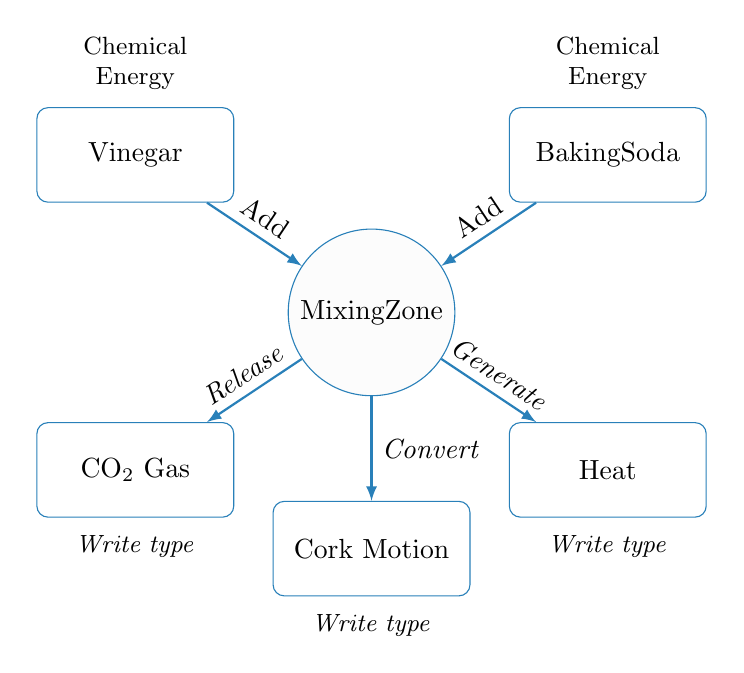
\begin{tikzpicture}[
    chemical/.style={draw=primaryblue, circle, minimum size=2cm, fill=lightgray!30},
    process/.style={draw=primaryblue, rectangle, rounded corners, minimum width=2.5cm, minimum height=1.2cm, fill=white},
    arrow/.style={thick, ->, >=latex, draw=primaryblue},
    note/.style={draw=none, fill=none, text width=2.5cm, align=center, font=\small}
]
% Central reaction
\node[chemical] (mix) at (0,0) {Mixing\\Zone};

% Inputs
\node[process] (vinegar) at (-3,2) {Vinegar};
\node[process] (soda) at (3,2) {Baking\\Soda};

% Outputs
\node[process] (gas) at (-3,-2) {CO$_2$ Gas};
\node[process] (motion) at (0,-3) {Cork Motion};
\node[process] (heat) at (3,-2) {Heat};

% Arrows
\draw[arrow] (vinegar) -- node[sloped, above] {Add} (mix);
\draw[arrow] (soda) -- node[sloped, above] {Add} (mix);
\draw[arrow] (mix) -- node[sloped, above] {\textit{Release}} (gas);
\draw[arrow] (mix) -- node[right] {\textit{Convert}} (motion);
\draw[arrow] (mix) -- node[sloped, above] {\textit{Generate}} (heat);

% Input/Output labels
\node[note, above=0.1cm] at (vinegar.north) {Chemical\\Energy};
\node[note, above=0.1cm] at (soda.north) {Chemical\\Energy};
\node[note, below=0.1cm] at (gas.south) {\textit{Write type}};
\node[note, below=0.1cm] at (motion.south) {\textit{Write type}};
\node[note, below=0.1cm] at (heat.south) {\textit{Write type}};

\end{tikzpicture}
\end{center}

Fill in the missing energy types and complete these questions:
\begin{enumerate}[label=\alph*)]
\item What type of energy is stored in the vinegar and baking soda? \rule{5cm}{0.5pt}
\item Name two forms of energy released in this reaction: \rule{8cm}{0.5pt}
\item Where does the energy to move the cork come from? \rule{8cm}{0.5pt}
\end{enumerate}

\item The video showed Bill Nye exercising. Describe the energy transformations that occur in your body during exercise:\\
\rule{\textwidth}{0.5pt}
\end{enumerate}
\end{conceptbox}

\vspace{1em}

\begin{conceptbox}[Part 3: Real-World Applications]
\begin{enumerate}[label=\arabic*., start=6, itemsep=8pt]
\item List three ways humans use electrical energy in daily life:
\begin{itemize}[label=$\square$]
\item \rule{0.8\textwidth}{0.5pt}
\item \rule{0.8\textwidth}{0.5pt}
\item \rule{0.8\textwidth}{0.5pt}
\end{itemize}

\item Match these energy sources with their type:\\[6pt]
\begin{tabular}{ll}
Coal \rule{2cm}{0.5pt} & A. Renewable\\
Wind \rule{2cm}{0.5pt} & B. Nuclear\\
Uranium \rule{2cm}{0.5pt} & C. Fossil Fuel\\
Solar \rule{2cm}{0.5pt} & D. Renewable
\end{tabular}
\end{enumerate}
\end{conceptbox}

\vspace{1em}

\begin{conceptbox}[Part 4: Energy Conservation]
\begin{enumerate}[label=\arabic*., start=8, itemsep=8pt]
\item Why is it important to conserve energy? Give two reasons:\\
1. \rule{0.9\textwidth}{0.5pt}\\[4pt]
2. \rule{0.9\textwidth}{0.5pt}
\end{enumerate}
\end{conceptbox}

\vspace{1em}

\begin{conceptbox}[Part 5: Critical Thinking]
\begin{enumerate}[label=\arabic*., start=9, itemsep=8pt]
\item Design an experiment that demonstrates an energy transformation.\\[6pt]
Materials needed: \rule{0.82\textwidth}{0.5pt}\\[4pt]
Steps: \rule{0.92\textwidth}{0.5pt}\\
\rule{\textwidth}{0.5pt}\\[4pt]
Expected results: \rule{0.84\textwidth}{0.5pt}\\[4pt]
Energy transformation occurring: \rule{0.75\textwidth}{0.5pt}

\item \textbf{Bonus Question:} How does your body transform the chemical energy from food? List two ways:\\
1. \rule{0.9\textwidth}{0.5pt}\\[4pt]
2. \rule{0.9\textwidth}{0.5pt}
\end{enumerate}
\end{conceptbox}

\end{document}